\documentclass[xcolor=dvipsnames,10pt]{beamer}
% ********** Styl prezentacji **********
\mode<presentation>
{
%\usetheme{Frankfurt}
%\usetheme{Copenhagen}
\usetheme{Madrid}
 %\usetheme{lankton-keynote}
 %Copenhagen
}
%\usepackage{amsmath}
%\usepackage{amsthm}
%\usepackage{amsfonts}
\usepackage{color}
\usepackage{draftwatermark}
%\usepackage{listings}
%\lstset{language=C++}
%\usepackage{lscape} 
%\usepackage{float}
%\usepackage{graphicx}
\usepackage{caption}
\usepackage{subcaption}
%\usepackage{multimedia}
% common reference commands
\renewcommand{\Re}{\textrm{Re}}
\newcommand{\Pe}{\textrm{P\'e}}
\renewcommand{\Pr}{\textrm{Pr}}
\newcommand{\eqt}[1]{Eq.~(\ref{#1})}                     % equation
\newcommand{\fig}[1]{Fig.~\ref{#1}}                      % figure
\newcommand{\tbl}[1]{Table~\ref{#1}}                     % table
%\usepackage{movie15}
%\usepackage{hyperref}
%\usepackage{multimedia}
\usepackage[]{media9}
%\usepackage{filecontents,hyperref,listings}
\newcommand{\resi}{R}
\newcommand{\resinew}{\widetilde{\resi}}
\newcommand{\resisource}{\widetilde{\resi}^{source}}
\renewcommand{\div}{\vec{\nabla}\! \cdot \!}
\newcommand{\grad}{\vec{\nabla}}
\newcommand{\divv}[1]{\vec{\nabla}^{#1}\! \cdot \!}
\newcommand{\gradd}[1]{\vec{\nabla}^{#1}}
\newcommand{\mbold}[1]{\boldsymbol#1}
\newcommand{\norm}{\textrm{norm}}
%

\newcommand{\tcr}[1]{\textcolor{red}{#1}}

%\setbeamertemplate{footline}[frame number]
%\title{Extension of the entropy viscosity method to low Mach regime and the seven equations model.}
%\title{Extension of the entropy viscosity method to low Mach regime and the seven equations model.}
%\author{Marc-Olivier Delchini}
%
\begin{document}
%
%\begin{frame}
%\maketitle
%\end{frame}
%\begin{frame}
%\begin{center}
%Extension of the entropy viscosity method to the low Mach Euler equations and the seven-equation two-phase model.
%\begin{center}
%by \\
%Marc-Olivier Delchini
%\end{center}
%\today \\
%
%Co-chairs: J. Ragusa\footnote{Nuclear Engineering Department, Texas A\&M University.} and J.L. Guermond\footnote{Department of Mathematics, Texas A\&M University.}. \\
%Committee members: J. Morel\footnotemark[1], Y. Hassan\footnotemark[1] and R. Berry\footnote{Idaho National Laboratory.}. \\
%Substitute: R. McClarren
%\end{center}
%\end{frame}
%
%\begin{frame}
%	\frametitle{Outline:}
%	\tableofcontents
%\end{frame}
%************************************************
\section{Numerical results}
\begin{frame}{A simple Pressurized Nuclear Reactor (PWR) model}
\begin{block}{The model}
\begin{itemize}
\setlength{\itemsep}{10pt}
\item A single $1$-D pipe of cross section $A=7.845 \times 10^{-5}$ $m^2$ and length $L = 3.865$ $m$.
\item Wall friction ($f=0.01$) and gravity forces.
\item Wall-heat source $Q_w = h_t p_w (T_{liq} - T_w)$ with $h_t = 5.33 \times 10^4$ $W/m$, $p_w = 2.82$ $mm$.
\item Wall temperature $T_w$ is a function of space and computed from the model available in RELAP-7: fuel, gap and clad with a constant power $P = 7.7 \times 10^3$ $kW / m^3$.
\item Inlet BC: specify total enthalpy ($H$) and momentum ($\rho u$).
\item Outlet BC: static pressure boundary with $P_s = 155$ $bar$.
\end{itemize}
\end{block}
\end{frame}
%************************************************
\begin{frame}{Discretization and stabilization methods}
\begin{block}{Discretization}
\begin{itemize}
\item Uniform mesh.
\item Second-order accurate implicit temporal integrator (BDF2).
\item Run until steady state is reached with a CFL of $100$.
\item Use a hard-coded Jacobian matrix as a preconditioner.
\end{itemize}
\end{block}
\begin{block}{Stabilization methods}
The code is run with three different statibilization methods for comparison:
\begin{itemize}
\item run with the entropy-viscosity method (EV).
\item run with SUPG.
\item run with first-order viscosity i.e. $\mu = \mu_{max}$ (FO).
\end{itemize}
\end{block}
\end{frame}
%************************************************
\begin{frame}{PWR: temperature steady-state profiles}
\begin{figure}
    \centering
    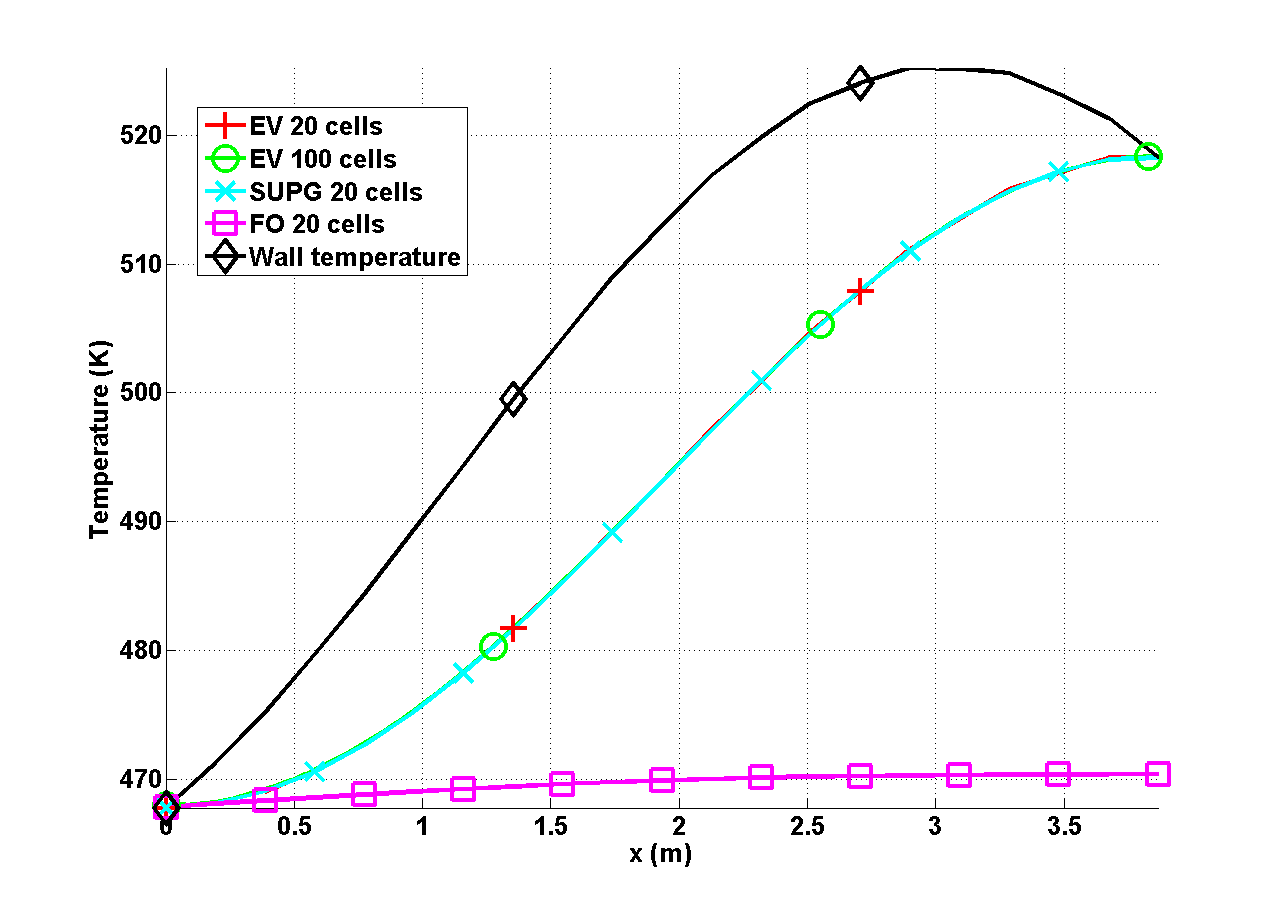
\includegraphics[width=0.98\textwidth]{plots/PWR_stt_temperature.png}
\end{figure}
\end{frame}
%************************************************
\begin{frame}{PWR: pressure steady-state profiles}
\begin{figure}
    \centering
    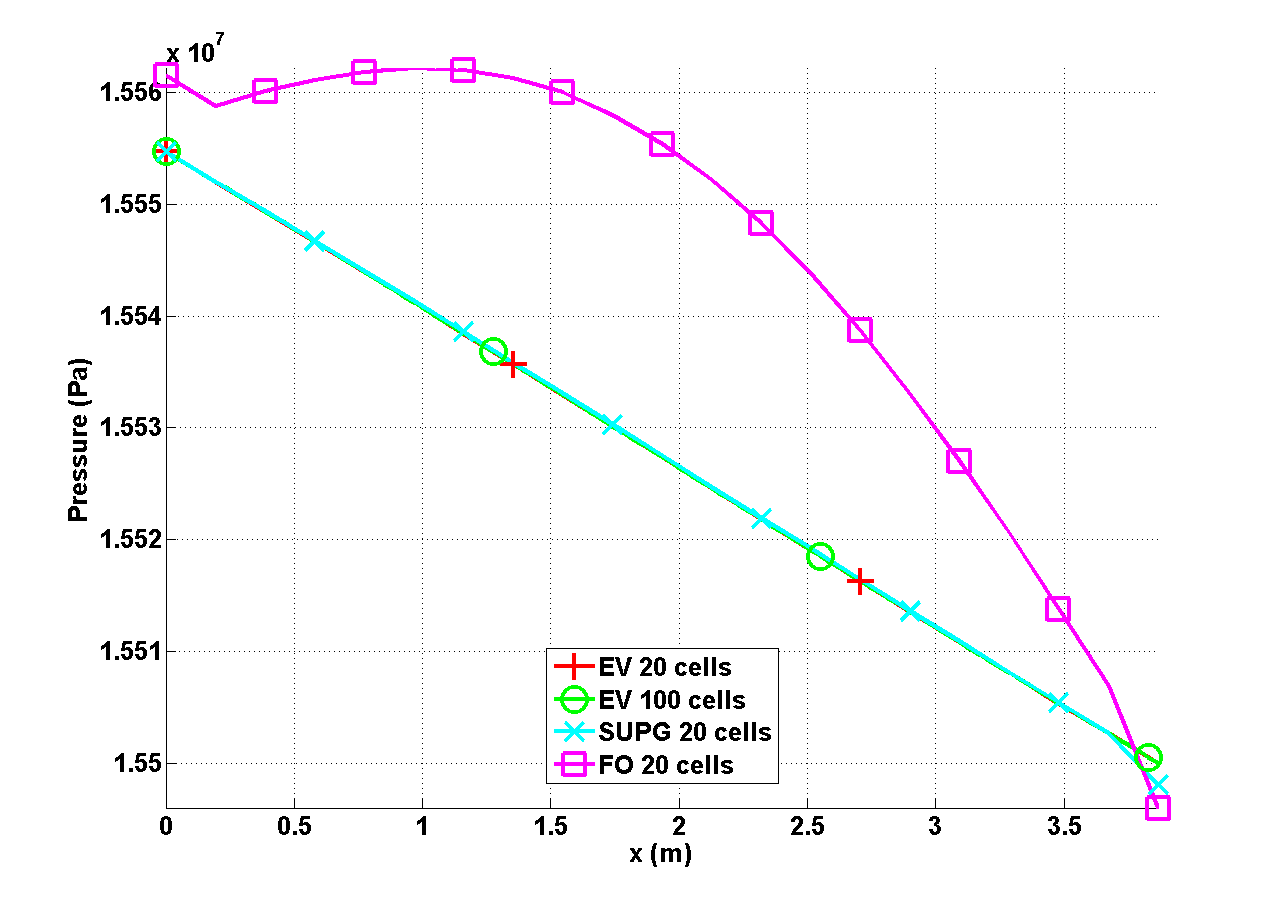
\includegraphics[width=0.98\textwidth]{plots/PWR_stt_pressure.png}
\end{figure}
\end{frame}
%************************************************
\begin{frame}{PWR: velocity steady-state profiles}
\begin{figure}
    \centering
    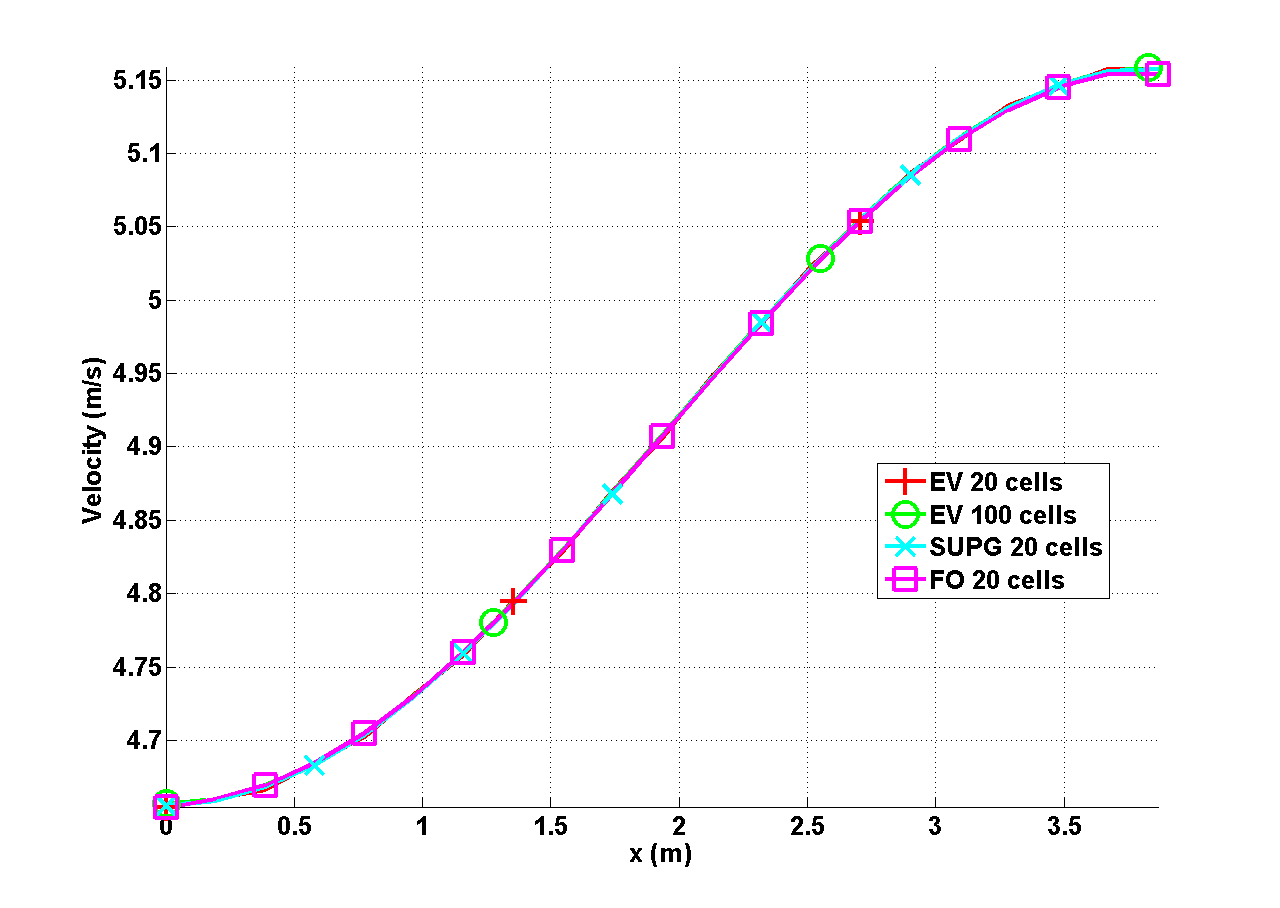
\includegraphics[width=0.98\textwidth]{plots/PWR_stt_velocity.png}
\end{figure}
\end{frame}
%************************************************
\begin{frame}{PWR: viscosity steady-state profiles}
\begin{figure}
    \centering
    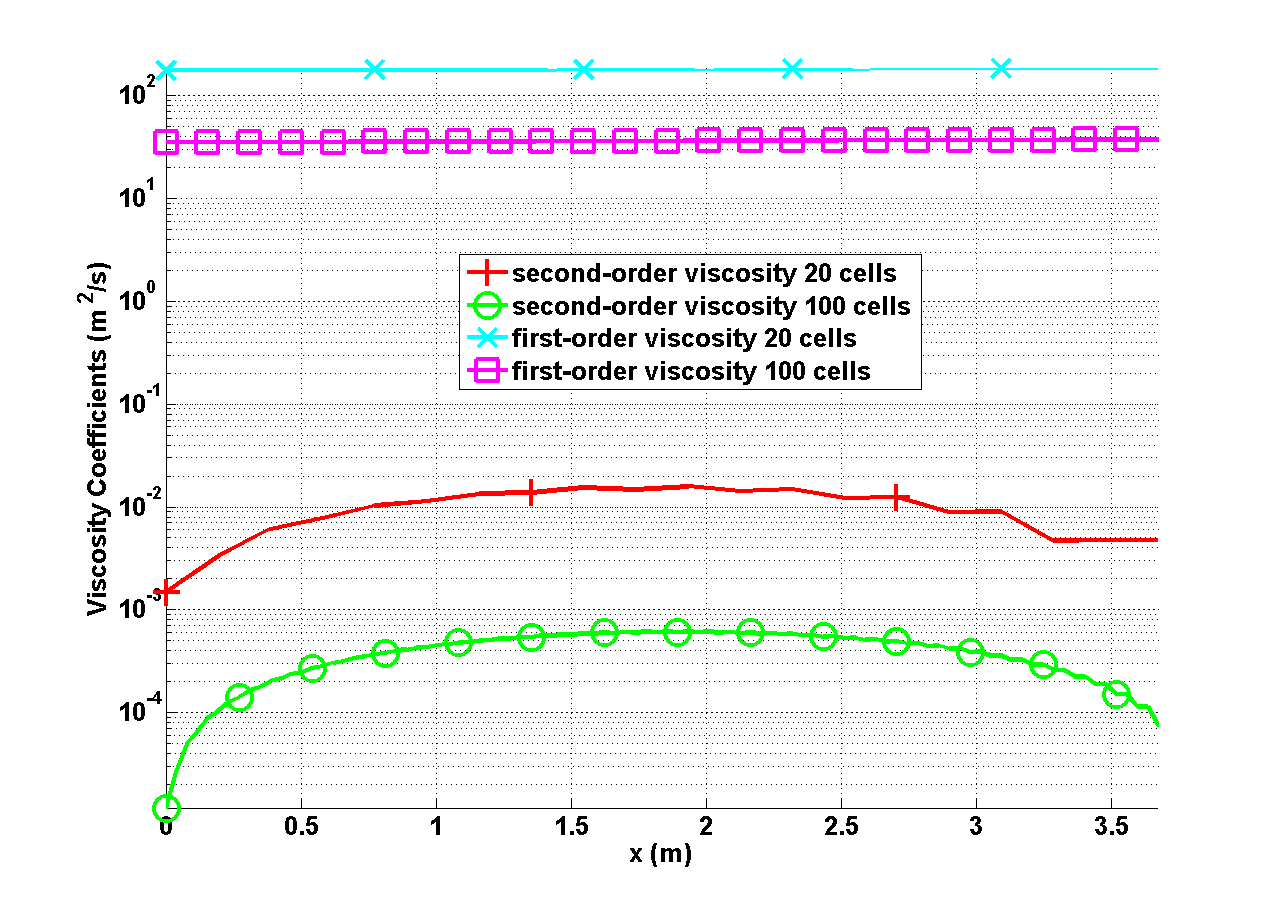
\includegraphics[width=0.98\textwidth]{plots/PWR_stt_viscosity.png}
\end{figure}
\end{frame}
%************************************************
\begin{frame}{PWR: mass flux steady-state profiles}
\begin{figure}
    \centering
    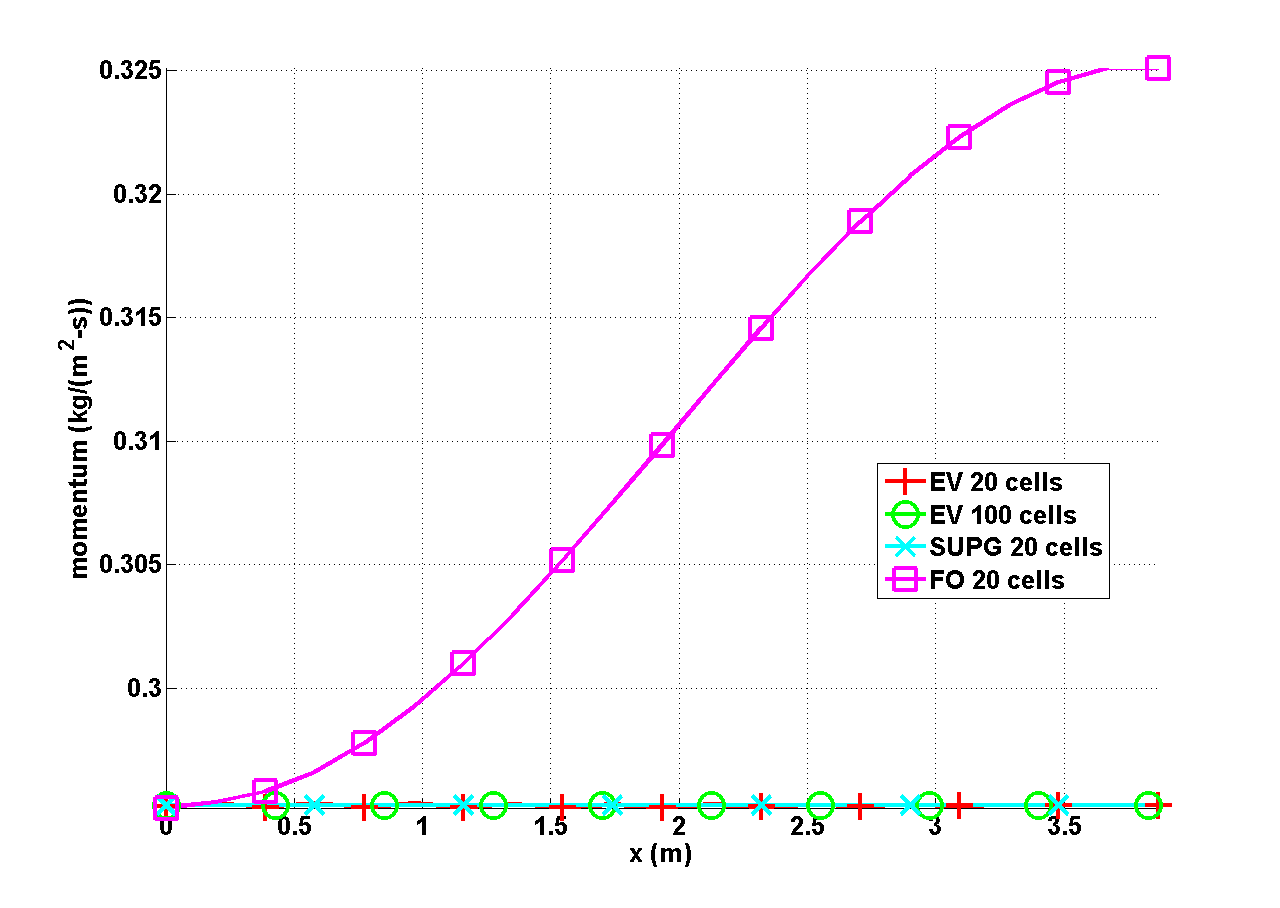
\includegraphics[width=0.98\textwidth]{plots/PWR_stt_momentum.png}
\end{figure}
\end{frame}
%************************************************
\end{document}